\documentclass[conference]{ieeeconf}
\IEEEoverridecommandlockouts
% The preceding line is only needed to identify funding in the first footnote. If that is unneeded, please comment it out.
\usepackage{cite}
\usepackage{amsmath,amssymb}
\usepackage{booktabs}
% \usepackage{caption}
\usepackage[ruled,linesnumbered]{algorithm2e}
\usepackage{graphicx}
\usepackage{subcaption}
\usepackage{textcomp}
\usepackage{xcolor}
\usepackage{microtype}
\usepackage{stmaryrd}

%WARNINGS
\usepackage{silence}
\WarningsOff



%MACROS
\newcommand{\powerset}[1]{2^{#1}}
\newcommand{\R}{\mathbb{R}}
\newcommand{\N}{\mathcal{N}}
\newcommand{\A}{\mathcal{A}}
\newcommand{\X}{\mathcal{X}}
\newcommand{\I}{\mathcal{I}}
\renewcommand{\P}{\mathcal{P}}
\renewcommand{\SS}{\mathcal{S}}
\newcommand{\G}{\mathcal{G}}
\newcommand{\E}{\mathcal{E}}
\newcommand{\D}{\mathcal{D}}
\newcommand{\Pref}{\mathsf{Pre}}
\renewcommand{\L}{\mathcal{L}}
\newcommand{\prefers}{\succsim}
\newcommand{\profile}{\boldsymbol{\pi}}
\newcommand{\metaprefers}{\sqsupseteq}
\newcommand{\indif}{\sim}
\newcommand{\join}{\vee}
\newcommand{\meet}{\wedge}
\newcommand{\bigjoin}{\bigvee}
\newcommand{\bigmeet}{\bigwedge}
\renewcommand{\leq}{\leqslant}
\renewcommand{\geq}{\geqslant}
\newcommand{\graph}{\mathcal{G}}
\newcommand{\edges}{\mathcal{E}}
\newcommand{\Act}{\mathcal{A}ct}
\DeclareMathOperator{\Atoms}{At}
\DeclareMathOperator{\cl}{cl}
\DeclareMathOperator{\Cl}{Cl}
\DeclareMathOperator{\Fix}{Fix}
\DeclareMathOperator{\Pre}{Prefix}
\DeclareMathOperator{\Post}{Suffix}
\DeclareMathOperator{\lfp}{lfp}
\DeclareMathOperator{\gfp}{gfp}
\DeclareMathOperator{\Aggregate}{Aggregate}
\DeclareMathOperator{\Median}{Median}
\DeclareMathOperator{\Permute}{Permute}

%Multi-Set Notation
\usepackage{scalerel}
\usepackage{stackengine}
\newcommand\doublelcurly{\stackengine{0pt}{\lbrace}{\kern-0.3ex\lbrace}{O}{l}{F}{F}{L}}
\newcommand\doublercurly{\stackengine{0pt}{\rbrace}{\kern-0.3ex\rbrace}{O}{l}{F}{F}{L}}
\newcommand\multiset[1]{\doublelcurly #1 \doublercurly}

%THEOREMS
\newtheorem{theorem}{Theorem}
\newtheorem{lemma}{Lemma}
\newtheorem{corollary}{Corollary}
\newtheorem{proposition}{Proposition}
\newtheorem{definition}{Definition}
\newtheorem{assumption}{Assumption}
\newtheorem{example}{Example}
\newtheorem{axiom}{Axiom}
\newtheorem{problem}{Problem}
\newtheorem{remark}{Remark}

\begin{document}

\title{\bf Preference Dynamics \textcolor{red}{title?}}

\author{Hans Riess, Gregory Henselman-Petrusek, Michael C.~Munger, Robert Ghrist, Zachary I.~Bell, and Michael M.~Zavlanos% <-this % stops a space
\thanks{Hans Riess is with the Department of Electrical \& Computer Engineering, Duke University. Email: {\tt hans.riess@duke.edu} (corresponding author).}%
v\thanks{Gregory Henselman-Petrusek is with the Pacific Northwest National Labratory.}%
\thanks{Michael Munger is with the Department of Economics and the Deparment of Political Science, Duke University.}%
\thanks{Robert Ghrist is with the Department of Electrical \& Systems Engineering, University of Pennsylvania.}%
\thanks{Zachary Bell is with the Air Force Research Laboratory, Eglin AFB.}%
\thanks{Michael Zavlanos is with the Department of Mechanical Engineering \& Material Science, Duke University.}%
}
\maketitle

\begin{abstract}
Preferences, fundamental in all forms of strategic behavior and collective decision-making, in their raw form, are an abstract ordering on a set of alternatives. Agents, we assume, revise their preferences as they gain more information about other agents or the requirements of a human supervisor (or society). Exploiting the ordered algebraic structure of preferences,  we introduce a decentralized preference-aggregation mechanism for heterogeneous agents distributed over a network and characterize the equilibria of the resulting global preference dynamics. The mechanism we design takes into account both external influence of other agents' preferences, by interacting with other agents, as well as the maintenance of internal coherence. We present numerical simulations demonstrating our preliminary results.
\end{abstract}

% \begin{IEEEkeywords}
% component, formatting, style, styling, insert
% \end{IEEEkeywords}

%%%%%%%%%%%%%%%%%%%%%%%%%%%%%%%%%%%%%%%%%%%%%%%%%%%%%%%%%%%%%%%%%%%%%%%%%%%%%%%%%%%%%%%%%%
\section{Introduction}

In their traditional use in economics and social science, preferences are commonly associated with human taste, want, or desire. Mathematically, however, a preference relation is a relative ordering of \emph{alternatives}, possible choices or options. Preferences are fundamental to collective decision---the \emph{social choice problem} problem \cite{choosingingroups}---involving collecting and aggregating input from voters, as well as \emph{non-cooperative games} \cite{gametheory} in which players take actions based on their preferences as well as, in effect, the preferences of other agents. In the social choice problem, a fundamental challenge is to design preference-aggregation mechanisms that satisfy certain criteria of fairness. When agents have limited communication or interaction with other agents, it is not feasible to aggregate preferences in a centralized or even synchronous manner. Worse, even if preferences are centrally gathered without strategic manipulation \cite{gibbard1973,satterthwaite1975}, faithfully representing preferences of a group of agents by a single aggregate preference is well-known to be a paradox, in the widely cited Impossibility Theorem \cite{arrow2012}. In a non-cooperative game, players are assumed from the outset to have preferences on the set of action profiles, tuples of actions indexed by players to be taken in the game. 

The focus of this paper is neither how choices are made in groups nor how players take actions based. Instead, our analysis, is focused on the emergent formation of the preferences themselves, \emph{preference dynamics}. While assuming preferences \emph{a priori} may sometimes be a neccesary convenience, it is arguably unrealistic to assume, as often assumed, that every pair-wise comparison of alternatives has been made by an agent. Furthermore, it is unrealistic to assume, depending on the setting, that fully-revealed preferences known to the ballot-reviewer (voting theory), or common knowledge to, depening on the setting to other agents (game theory), i.e.~every agent knows every other agent's preferences, every agent knows that every agent knows every other agent's preference, etc. We relax both common assumputions by supposing that preferences are incomplete (i.e.~every pair of alternatives need not be compared) and agents are organized in a network structure.


We also challenge how preferences are reprsented. Utility functions represent some classes of preference relations, however, others are unrepresentable \cite{Beardon2002}. If preferences are represented by utility functions, techniques in distributed optimization apply to the social choice problem, i.e.~finding an alternative that maximizes the social welfare, i.e.~sum of utilities of agents. Nevertheless, utility functions, which represent complete and transitive preferences, are not capable of capturing the distinction between indifference between two alternatives, i.e.~one is not better than the other, and indecisiveness, i.e.~the agent has not made up its mind between the two alternatives or faced a choice between the two alternatives \cite{eliaz2006}. Furthermore, decision making in the real-world is often accompanied by conflicting or unresolved preferences \cite{levi1990}. The present paper offers a novel methodology for aggregating incomplete preferences in a robust and decentralized manner.

While it is widely believed that preferences are stable, and that apparent fluctuations in preferences are the result of changes in information (e.g.~prices), not the preferences themselves \cite{stigler1977}, it is also argued, to the contrary \cite{hansen1995}, that preferences can, in fact, change due to factors of external influence, e.g.~by other agents, and internal coherence, i.e.~altering inconsistent preferences. In our model of preference dynamics, we take into account both elements of preference change. Mechanisms of preference change include revision, contradiction, as well as addition and subtraction of alternatives \cite{hansen1995}. Our message-passing model of preference dynamics, based on the algebraic lattice structure of preference relations, incorporates elements of both revision (the join operation) and contraditions (the meet operation). Avoiding the chicken-or-the-egg, preference dynamics can be construed as either an explanation for how preferences are formed in the first place, or how confounding variables effect the perceived expression of preference. We also study the equilibria of preference dynamics: stable preferences.
% Formal models of preference change include revision, contradiction, as well as addition and subtraction of alternatives \cite{hansen1995}.

While preferences have been studied classically in the human domain, we now argue that preference dynamics extends in scope to non-human agents.
Intelligent multi-robot systems, for instance, making autonomous decisions about what tasks to perform as well as what paths to take to reach a target location, are, arguably, making their decisions based on preference. If robots make these decisions collaboratively, or even react to the decisions of other agents, they are also, in effect, dynamically aggregating preferences. In reinforcement learning (RL), especially unexplainable models, agents form implicit preferences based on performing actions that maximize rewards, although sometimes rewards and broader goals can become misaligned \cite{pan2022}, a phenomenon known as ``reward hacking.'' Several efforts \cite{?} have been made to design systems whose outcomes imitate human preference, but, in the absence of a human controller, it is a challenging problem to control preferences of autonomous agents. Our strategy to is design  mechanisms converging to stable preferences.

\paragraph*{Related work}

Recent efforts have approached consensus \cite{riess2022}, synchronization \cite{maxplussync}, and signal processing \cite{puschel} from the perspective of ordered sets, e.g.~lattices. Several authors have studied aggregation or consensus functions on lattices \cite{frenchdudes}, and there is a corpus of literature addressing the design of preference-aggregation mechanisms \cite{arrow2012}, but, to our knowledge, none have approached the problem of preference dynamics from either a decentralized or algebraic point-of-view. The several efforts to formalize classical consensus algorithms with lattice theory \cite{consensus}, motivated by data science, are restricted to a complete or star topology. Our treatment of preference dynamics is also closely related to opinion dynamics \cite{opinion}. Opinions are typically framed as numeric representations of likes or dislikes versus preferences which are relational objects.


%%%%%%%%%%%%%%%%%%%%%%%%%%%%%%%%%%%%%%%%%%%%%%%%%%%%%%%%%%%%%%%%%%%%%%%%%%%%%%%%%%%%%%%%%%
\section{Problem Formulation}

Suppose agents are collected in a finite set $\N = \{1,2,\dots,N\}$. Agents interact (e.g.~communicate) with other agents according to the topology of a fixed undirected graph $\graph = (\N,\E)$ where $\E$ is the set of pairs of agents $(i,j) \in \E$ such that Agent $i$ and Agent $j$ interact. For $i \in \N$, let $\N_i = \{ j~:~(i,j) \in \E\}$ denote the set of \emph{neighbors}. Agents form preferences over a fixed and a set of alternatives, $\A$. The set of all feasible preference relations over a fixed set of alternatives is collected in a set $\Pref(\A)$. Elements of a preference relation in $\Pref(\A)$ are written $a \prefers_i b$ (instead of as an ordered pair), and indexed by each agent $i \in \N$. For example, $a \prefers_i b$ means \emph{Agent $i$ prefers Alternative $a$ to Alternative $b$}. We say that an agent is indifferent between two alternatives, written $a \indif_i b$, if both $a \prefers_i b$ and $b \prefers_i a$.

For purposes of illustration, we consider three examples of agents, alternatives, preferences and graphs from different domains.

\begin{example}[Trade]
    Suppose consumers and producers have various levels of supply and demand for goods $\{1,2,\dots,d\}$. The alternative set consists of  bundles-of-goods, positive quantities of each alternative, constrained by the divisibility or availabilities of each alternative, $\A \subseteq \R^{d}_{+}$. Preferences consist of comparisons between bundles of goods; it is often assumed that preferences are monotone, i.e.~more of a good is always preferred to less. The graph is a bipartite graph whose edges consist of pairs of consumers and producers who engage in trade.
\end{example}
\begin{example}[Multi-Agent RL]
    Suppose agents take actions from a set $\Act$ via a local policy $\mu_i: \prod_{i \in \N} \SS_i \to \Act$ where $\SS_i$ is the set of states of Agent $i$. The alternatives $\A$ are the set of policies. An agent forms preferences over policies, for instance, by maximizing the cumulative discounted reward $\sum_{t=0}^{\infty} \gamma^t r_{i,t}(\mathbf{s},a)$. The graph consists of pairs of agents whose policy functions are coupled.
\end{example}
\begin{example}[Teams of Robots]
    Suppose a team of autonomous robots are collaboratively performing tasks. Agents form preferences over tasks---the alternatives---based on the skills required to complete the task, the number of agents needed to help with the task, as well as the time it will take to complete the task. The graph consists of an \emph{ad hoc} wireless communication network which agents utilize to coordinate tasks.
\end{example}

%DO WE NEED TO ASSUME THERE ARE FINITELY MANY ALTERNATIVES?


We assume that agents' preferences satisfy the following axioms.
\begin{assumption}[Reflexivity] \label{ass:reflexivity}
    The preference $\prefers_i$ satisfies $a \prefers_i a$ for all $a \in \A$ and for all $i \in N$.
\end{assumption}

Irreflexive preferences are said to be \emph{strict} while reflexive preferences are \emph{weak}. One can always obtain a strict preference from a weak preference by defining $a \succ_i b$ if and only $a \succeq_i b$ and $b \not\succeq_i a$.

\begin{assumption}[Transitivity]\label{ass:transitivity}
    For all $i \in \N$ and for all $a, b, c \in \A$ such that $a \prefers_i b$ and $b \prefers_i c$, it is necessarily true that also $a \prefers_i c$.
\end{assumption}

Intransitive preferences are inconsistent. We remark that we do \emph{not} assume preferences are complete, i.e.~we do not assume for all $a,b \in \A$, $a \prefers_i b$ or $b \prefers_i a$. Thus, an agent may be indecisive, or, alternatively, limited information about an agent's preferences is known. 

Let $\profile = \left( \prefers_1, \prefers_2, \dots, \prefers_N \right)$ be a tuple of preference relations indexed by each agent, called a \emph{preference profile}. We study how a preference profile changes based on interactions between agents. If $J \subseteq \N$ is a group of agents, we let $\pi_{J}$ be the preference profile restricted the indices in $J$; in particular, $\pi_j$ is simply $\prefers_j$. Agents update their preferences in a series of rounds indexed by discrete time instants $t=0,1,2,\dots$ according to coupled dynamics
\begin{align}
    \begin{aligned}
        \pi_i(t+1) &=& F_i \bigl( \profile(t) \bigr)  \\
        \pi_i(0) &=& \pi_{i,0}
    \end{aligned}, \quad i \in \N
    \label{eq:pi-dynamics}
\end{align}
where $F_i: \Pref(\A)^N \to \Pref(\A)$ is an iterative map.

The first problem we address in this paper is modeling preference dynamics over a graph. Unlike opinion dynamics, in which standard dynamical systems theory can at least model how likes and dislikes on topics change over time, preference dynamics requires some level of algebraic sophistication. Thus, notions of structure-preserving maps as well as binary operations on preference relations are introduced with no assumed background (Section \ref{sec:lattices}). If we suppose agents update their preferences according to dynamics of the form \eqref{eq:pi-dynamics}, what sorts maps $F_i$, preserving the structure of preferences, model the process of preference revision? In our design of $F_i$, we focus on several aspects of preference change including agents having different ``personalities'' informing how they communicate, aggregate, and update preferences, agents fairly incorporating new comparisons into their preferences given a high enough level of consensus, all the while maintaining the consistency (transitivity) of their own preferences.

The second problem we address is a computational one. Suppose preferences evolve according to \eqref{eq:pi-dynamics} and the iterative maps $F_i$ are known. \textcolor{red}{Need to finish!}

% \begin{table}
% \centering
% \caption{}
% \label{table:notation}
% \begin{tabular}{p{5cm}c}
% \toprule
% Concept & Notation \\
% \midrule
% Agent, & $i \in \N$ \\
% Alternative, & $a \in \A$ \\
% Preference, & $a \prefers_i b$ \\
% Preference profile, & $\profile = \left(\pi_1,\pi_2,\dots,\pi_N\right)$ \\
% Metapreference, & $\pi \metaprefers \pi'$ \\
% \bottomrule
% \end{tabular}
% \end{table}

\section{Preference Lattices}
\label{sec:lattices}
%%%%%%%%%%%%%%%%%%%%%%%%%%%%%%%%%%%%%%%%%%%%%%%%%%%%%%%%%%%%%%%%%%%%%%%%%%%%%%%%%%%%%%%%%%

The set of transitive-reflexive preferences on a fixed set of alternatives is an algebraic structure known as an (order) lattice \cite{birkhoff1940}. We exact this observation and interpret the meaning of the lattice operations \emph{meet} and \emph{join} as binary operations on preferences. Our interpretation for how agents \emph{amalgamate}, i.e.~combine, preferences is reminiscent, in fact a special case of, the calculus of relations \cite{tarski1941}, a series of rules for manipulating (general) binary relations. We begin with some definitions from order theory \cite{roman2008}.

\subsection{Ordered Sets}

A \emph{preorder} is a set $\P$ with a relation $\precsim$ satisfying the axioms of transitivity and reflexivity. Preferences, we assume, are preorders, and we will use both terms interchangeably. A \emph{partial order} is a a preorder, with an order usually written $\preceq$ satisfying a third axiom, called anti-symmetry: if $\pi_1 \preceq \pi_2$ and $\pi_2 \preceq \pi_1$, then $\pi_1 = \pi_2$. Note do not assume preferences satisfy the third axiom because we want to model indifference between alternatives. Hence, we write $\pi_1 \prec \pi_2$ whenever $\pi_1 \preceq \pi_2$, but $\pi_2 \not \preceq \pi_1$.

A map $f: \P \to \P$ between partial orders is \emph{monotone} if $\pi_1 \preceq \pi_2$ implies $f(\pi_1) \preceq f(\pi_2)$, \emph{inflationary} if $f(\pi) \succeq \pi$ for all $\pi \in \P$, and \emph{deflationary} if $f(\pi) \preceq \pi$ for all $\pi \in \P$. Note, inflationary or deflationary functions are not necessarily monotone. Let $\Fix(f) = \{ \pi \in \L: f(\pi) = \pi \}$ denote the set of fixed points, $\Pre(f) = \{ \pi \in \L : f(\pi) \preceq \pi\}$ the set of \emph{prefix points}, and $\Post(f) =\{ \pi \in \L : f(\pi) \succeq \pi\}$ the set of \emph{suffix points}. If they exist, let $\lfp(f)$ and $\gfp(f)$ denote the least and greatest fixed points, respectively.

Cartesian products of ordered sets $\P_1 \times \P_2 \times \cdots \times \P_N$ yield an ordered set under the \emph{product order}: $(\pi_1, \pi_2, \dots, \pi_N) \preceq (\pi_1', \pi_2', \dots, \pi_N')$ if and only if $\pi_i \preceq \pi'_i$ for all $i = 1,2,\dots, N$. 

% \begin{lemma} \label{lem:compose-produt}
%     Suppose $f_1: \P_1 \to \P_3$ and $f_2: \P_2 \to \P_4$ are monotone.  Then, $f: \P_1 \times \P_2 \to \P_3 \times \P_4$, defined $f(\pi_1,\pi_2) = (f_1(\pi_1),f_2(\pi_2))$ is monotone in the product order. If $\P_2 = \P_3$, then, the composition $f_2 \circ f_1: \P_1 \to \P_3$ is monotone.
% \end{lemma}

Ordered sets on their own have no algebraic structure. Lattices are partial orders with a rich algebraic structure given by two merging operations called ``meet'' and ``join.''
 
\begin{definition} \label{def:lattice}
    An \emph{lattice} is a partial order $(\L, \preceq)$ such that, for any two elements $\pi_1, \pi_2 \in \L$ the following operations,
    \begin{align*}
        \begin{aligned}
        \pi_1 \meet \pi_2 &=& \max\{ \pi \in \L: \pi \preceq \pi_1,~\pi \preceq \pi_2 \} \\
        \pi_1 \join \pi_2 &=& \min\{ \pi \in \L: \pi \succeq \pi_1,~\pi \succeq \pi_2 \},       
        \end{aligned},
    \end{align*}
    called \emph{meet} (greatest lower bound) and \emph{join} (least upper bound), exist. 
\end{definition}

We recall a set of properties that characterize lattices as ordered algebraic structures.

\begin{lemma} \label{lem:lattice-axiom} 
    Suppose $(\L,\preceq)$ is a lattice. Then, $\meet, \join: \L \times \L \to \L$ satisfy the following:
    \begin{itemize}
        \item[(i)] \emph{commutativity}, i.e.~$\pi_1 \meet \pi_2 = \pi_2 \meet \pi_1$, $\pi_1 \join \pi_2 = \pi_2 \join \pi_1$;
        \item[(ii)] \emph{associativity}, i.e. {\small $\pi_1 \meet (\pi_2 \meet \pi_3) = (\pi_1 \meet \pi_2) \meet \pi_3$}, etc.;
        \item[(iii)] \emph{idempotence}, i.e.~$\pi \meet \pi = \pi \join \pi =  \pi$;
        \item[(iv)] \emph{absorption}, i.e.~$\pi_1 \join \left( \pi_1 \meet \pi_2 \right) = \pi_1 \meet \left( \pi_1 \join \pi_2 \right) = \pi_1$;
        \item[(v)] \emph{monotonicity}, i.e. $\join$ and $\meet$ are monotone in both arguments.
    \end{itemize}
\end{lemma}
\begin{proof}
    See \cite[\S I.4 Lemma 1, \S I.5 Lemma 3]{birkhoff1940}.
\end{proof}

Given variables $\pi_1,\pi_2,\dots,\pi_n$, a \emph{lattice polynomial} is a term in the language $\pi_1,\pi_2,\dots,\pi_n~\vert~\pi \meet \pi'~\vert~\pi \join \pi'$, i.e.~an expression formed by finite application of these symbols. Suppose $\L$ is  lattice. Then, a lattice polynomial $p$ defines an evaluation map $\mathrm{ev}_p: \L^n \to \L$ by substituting an element of $\L$ into each variable of $p$.

\begin{lemma} \label{lem:lattice-polynomial}
    Suppose $p$ is a lattice polynomial. Then, $\mathrm{ev}_p(\pi_1,\pi_2,\dots,\pi_n)$ is monotone in the product lattice $\L^n$.
\end{lemma}
\begin{proof}
    See \cite[\S I.5 Lemma 4]{birkhoff1940}.
\end{proof}

A lattice is \emph{complete} if, given an arbitrary indexing set $J$,
\begin{align}
    \begin{aligned}
        \bigmeet_{j \in J} \pi_i = \max\{\pi \in \L : \pi \preceq \pi_j~\forall i \in I\} \\
        \bigjoin_{j \in J} \pi_i = \min\{\pi \in \L : \pi \succeq \pi_j~\forall i \in I\}
    \end{aligned} \label{eq:complete lattice}
\end{align}
exist. In particular, $\bigmeet \emptyset = \top$, the \emph{maximum element}, and $\bigjoin \emptyset = \bot$, the \emph{minimum element}.

%Birkhoff Lemma 5.4

% \begin{lemma}\label{lem:lattice-poly}
%     Suppose $p$ is a lattice polynomial. Then, $p$ is monotone.
% \end{lemma}

\subsection{The Information Order}

Let $\Pref(\A)$ denote the set of preorders over a ground set $\A$, hereafter called \emph{preference relations}. We equip $\Pref(\A)$ with the partial order inherited from the inclusion order on the powerset of $\A \times \A$, which we call the \emph{information order}. Let $\pi_1, \pi_2 \in \Pref(\A)$. We write $\pi_1 \succeq \pi_2$, i.e.~{\it $\pi_1$ contains more information than $\pi_2$}, if $\pi_2$ is contained in $\pi_1$ as subsets of $\A \times \A$. The minimum element in the information order is the preference relation, written $\epsilon$, defined $a \prefers a$ for all $a \in \A$. An agent with this preference relation has not compared any alternatives. The maximum element, written $\iota$, in the information order satisfies $a \prefers b$ for all pairs $(a,b) \in \A \times \A$. An agent with this preference relation is indifferent between any two alternatives. In fact, indifference $a \sim b$ forms an equivalence relation. The set of preference relations over $\A$ contains the set of equivalence relations (or partitions) on $\A$. Thus, the information order defines a metapreference where richer (more indifference) preference relations are always preferred to sparser ones (more indecision).

If agents are to compare preferences, we want to ensure that the result of gathering the preferences of two or more agents and collecting them in a single aggregate preference will result in a transitive-reflexive preference as long as the individual preferences are transitive-reflexive (Assumption \ref{ass:reflexivity}-\ref{ass:transitivity}). This requires a unary operation known as a transitive-reflexive closure.
\begin{definition}
    Suppose $\pi \subseteq \A \times \A$. The \emph{transitive closure} of $\pi$ is the preference relation 
\begin{align}
    \pi^{\star} = \bigcup_{p=1}^{\infty} \overbrace{\pi \circ \pi \circ \cdots \circ \pi}^{p}, \label{eq:transitive-closure}
\end{align}
where $\pi \circ \pi = \{ (a \prefers b)~\vert~\exists c,~a \prefers c,~c \prefers b\}$. The \emph{transitive-reflexive closure} of $\pi$ is the preference relation $\pi^{+} = \left( \pi \cup \epsilon \right)^\star$.
\end{definition}

% The transitive-reflexive closure is an example of a \emph{closure operator}, i.e.~a map $\cl(-): \powerset{\X} \to \powerset{\X}$, given a set $\X$, such that
% \begin{enumerate}
%     \item $\cl(\cl(S)) = \cl(S)$ for all $S \in \powerset{\X}$;
%     \item $\cl(S) \supseteq S$ for all $S \in \powerset{\X}$;
%     \item $S \subseteq S'$ implies $\cl(S) \subseteq \cl(S')$.
% \end{enumerate}
% It is well-known that that the set of closed subsets
% \begin{align*}
%     \Cl(\X) = \{ S \in \powerset{\X}: \cl(S) = S\}
% \end{align*}
% with the order $(\Cl(\X), \subseteq)$ is a lattice.

The transitive closure as well as the union and intersection of preference relations are enough to specify the structure of a lattice.

\begin{theorem} \label{thm:complete-lattice}
    $(\Pref(\A), \succeq)$ is a complete lattice with meets and joins given by the following
    \leavevmode
    \begin{align}
 %    \begin{aligned}
 %        \pi_1 \meet \pi_2 &=& \pi_1 &\cap \pi_2& \\
 % \pi_1 \join \pi_2 &=&  \left(\pi_1  \right. &\left. \cup \pi_2  \right)^{+}
 %    \end{aligned}. \label{eq:join-meets}
    \begin{aligned}
        \bigmeet_{j \in J} \pi_j & = &\bigcap_{j \in J} \pi_j \\
        \bigjoin_{j \in J} \pi_j & = \biggl( &\bigcup_{j \in J} \pi_j \biggr)^{+}
    \end{aligned}.\label{eq:meets-joins}
\end{align}
\end{theorem}
\begin{proof}
    See Appendix.
\end{proof}

For a pair, $\pi_1 \meet \pi_2 = \pi_1 \cap \pi_2$ and $\pi_1 \join \pi_2 = \left( \pi_1 \cup \pi_2 \right)^{+}$. We briefly interpret the meet and join operations of the \emph{information lattice}. A preference $a \prefers b$ is in the meet $\pi_1 \meet \pi_2$ if and only if it is in both $\pi_1$ and $\pi_2$. Thus, the meet of two preference relations constitutes a consensus between them. The join is somewhat more subtle. For one, $\pi_1 \join \pi_2$ is the smallest transitive-reflexive relation containing $\pi_1 \cup \pi_2$. Theorem \ref{thm:complete-lattice} holds even if $\A$ is not finite. In the finite case, another interpretation exacts what it means for a pair-wise comparison to be in the join of two preference relations.
\begin{proposition} \label{prop:join}
    Suppose $\A$ is finite, and suppose $\pi_1, \pi_2 \in \Pref(\A)$. Then, $(a \prefers b) \in \pi_1 \join \pi_2$ if and only if either, (i) $(a \prefers b) \in \pi_1 \cup \pi_2$, or, (ii) there exist a chain
    \begin{align}
        a = c_0 \prefers_{j_1} c_1 \prefers_{j_2}  \cdots \prefers_{\ell-1} c_{j_{\ell-1}} \prefers_{j_\ell} c_{\ell} = b \label{eq:chain}
    \end{align}
    such that $\left( c_{m-1} \prefers_{{j_m}} c_{m} \right) \in \pi_1 \Delta \pi_2$ (symmetric difference).
\end{proposition}
\begin{proof}
    See Appendix.
\end{proof}

Thus, the join of two preference relations facilitates the rational, i.e.~transitive, conclusion of two agents having merged their preferences.

% \begin{remark}
%     We call the lattice $(\Pref(\A), \succeq)$ an ``information order'' due to the fact that an analogous order on the set of equivalence relations, i.e.~partitions, on a fixed set, which forms a proper subset of $\Pref(\A)$, is called an ``information order'' because of its relevance in information theory \cite{shannon}.
% \end{remark}
\begin{remark}
    It is also possible to design other lattice orders on $\Pref(\A)$. In this case, meets and joins have the following interpretation: the join of two preferences is the (unique) worst preference that is at least as good as both preference. Similarly, the meet of two preferences is the (unique) best preference such that both preferences are as least as good as it. We leave this approach to future work.
\end{remark}


%%%%%%%%%%%%%%%%%%%%%%%%%%%%%%%%%%%%%%%%%%%%%%%%%%%%%%%%%%%%%%%%%%%%%%%%%%%%%%%%%%%%%%%%%%
\section{Preference Dynamics}
\label{sec:dynamics}

In this section, we introduce a novel model of preference dynamics based on a message-passing framework. In that framework, we discuss possible message, aggregation and update rules based on the structure of the information lattice. Thus, in the spirit of opinion dynamic models, such as the DeGroot model \cite{degroot1974} or the Hegselmann-Krause model \cite{hegselmann2002}, we proceed by defining simple rules for agents aggregating information by collecting and processing the preference relations of neighboring agents, $j \in \N_i$, with respect to the topology of $\G = (\N,\E)$.

\subsection{The Model}

We model how agents update their prefences in the course of a round in the manner of a message-passing algorithm (Algorithm \ref{alg:messsage-passing}). The algorithm follows a familiar gather-scatter paradigm \cite{dudzik}. Agents send messages to their neighbors in each round (Line 4). Messages, we assume, consist of applying a function $\psi(\pi_i,\pi_j)$ sending two preference relations $\pi_i, \pi_j, j \in \N_i$ to a another preference relation on the same alternative set.
% If $\psi(\pi_i,\pi_j) = \pi_j$, then Agent $j$ represents their preference faithfully and communicates it to Agent $i$. Otherwise, Agent $j$ alters its preference, (possibly) based on an estimate of $\pi_i$ as well as $\pi_j$. In an allusion to the diffusion equations, message passing algorithms with messages  $m_j \gets \psi(\pi_j)$ have been referenced as \emph{isotropic} \cite{dudzik}.
Next, after collecting the messages as they are received (Line 5-6), agents aggregate the messages into a single preference relation (Line 8). Finally, the agents update their preference as a result of the aggregation and their prior-held preference via a function  $\varphi(\pi_i,\cdot)$. Algorithm \ref{alg:messsage-passing}, thus, can be summarized by a choice of a function
\begin{align}
    F_i(\profile) = \varphi\Bigl(\pi_i, \Aggregate{\left[ \psi(\pi_j, \pi_i)\right]_{j \in \N_i}} \Bigr) \label{eq:message-passing}
\end{align}
for the local preference updates $\pi_i(t+1) = F_i\left( \profile(t) \right)$.

\subsection{Examples}

For the remainder of this section, we discuss candidates for the functions $\psi, \Aggregate(\cdot)$, and $\varphi$, noting how various personalities of agents affect the choice of functions. In particular, we address functions that utilize the lattice structure of the information order.

\begin{algorithm}[t]
\caption{$\mathsf{RevisePreference}$} \label{alg:messsage-passing}
\SetKwComment{Comment}{/* }{ */}
\KwData{Agent, $i \in \N$; preference, $\pi_i \in \Pref(\A)$;  message function, $\psi$; aggregation function, $\Aggregate(\cdot)$; update function, $\varphi$.}
\KwResult{Preference, $\pi_i \in \Pref(\A)$.}
$\mathcal{M} \gets [~]$ \\
\For{$j \in \N_i$}{
$\pi_j \gets \mathsf{Preference}(j)$ \\
Agent $j$ sends $\psi(\pi_i,\pi_j)$ to Agent $i$, \\
Agent $i$ receives $\pi_{\mathrm{mes}} \gets \psi(\pi_i,\pi_j)$, \\
Agent $i$ appends $\pi_{\mathrm{mes}}$ to $\mathcal{M}$,
}
$\pi_{\mathrm{agg}} \gets \mathsf{Aggregate}\left( \mathcal{M} \right)$, \\
$\pi_i \gets \varphi(\pi_i, \pi_{\mathrm{agg}})$.
\end{algorithm}

\paragraph*{Messages}
Message functions $\psi(\pi_i,\pi_j)$ that are invariant to the first argument are said to be \emph{isotropic} because there is no feedback in the resulting ``diffusion'' process. In the isotropic case, if $\psi(\pi_j) = \pi_j$, Agent $j$ represents their preference faithfully and communicates it to Agent $i$. Such agents can be thought of as being honest. Dishonest agents misrepresent their true preferences with a non-trivial map $\psi: \Pref(\A) \to \Pref(\A)$. In the opinion dynamics literature \cite{hansen2021}, behaviors such as exaggerating opinions, restricting the topics of discussion, or lying can be represented by similar maps. We expect analogous behaviors to be modeled with appropriate transformations of preference relations. In the non-isotropic case, agents represent their preferences as a result of feedback. In the simplest instance, Agent $j$ could pretend its preference is the same as Agent $i$, i.e.~$\psi(\pi_j,\pi_i) = \pi_j$, but more complex feedback mechanisms are possible.

\paragraph*{Aggregation}
% It is commonly assumed in message-passing algorithms that the order messages are received has no bearing on the resulting aggregate preference \cite{?}. In the present case, this means that the identities of the agents are anonymous, or, at least, every neighbor $j \in \N_i$ is treated equally. The lattice structure of the information order on preferences provides a natural hierarchy of aggregation functions which we now examine. Since there is no way to ``average'' preferences numerically, the lattice median seems a good fit for an aggregation mechanism that can produce stable preference profiles. It is also obvious that lattice medians are invariant to permutations of the labels of the agents.
Aggregating preference relations accurately is a significant challenge. Fortunately, the lattice structure of the information order provides some reasonable choices. In our message-passing framework, sub-index the neighbor set, i.e. $\N_i = \{j_1,j_2,\dots,j_n\}$. Suppose $\Aggregate(\cdot): \bigcup_{n =1}^{N} \Pref(\A)^n \to \Pref(\A)$ is an aggregation function sending an $n$-tuple of preferences to an aggregate preference, $\Aggregate(\pi_{j_1},\pi_{j_2}, \dots, \pi_{j_n})$. We say $\Aggregate(\cdot)$ satisfies \emph{anonymity} if for all $n$-tuples,
\begin{align*}
    \Aggregate\left( \pi_{j_1},\dots,\pi_{j_n}\right) = \Aggregate\left( \pi_{\sigma(j_1)},\dots,\pi_{\sigma(j_n)}\right) \\ \forall \sigma \in \Permute(\{j_1,j_2,\dots,\j_n\}),
\end{align*}
 \emph{unanimity} if $\pi_{j} = \pi_{j'} = \pi$ for all $j, j' \in \{j_1,j_2,\dots,j_n\}$ implies 
\begin{align*}
    \Aggregate\left( \pi_{j_1},\pi_{j_2},\dots,\pi_{j_n}\right) = \pi, 
\end{align*}
and $r$-\emph{middle} if, given $1 \leq r \leq n$, the ordering $\pi_{j_1} \preceq \pi_{j_2} \preceq \cdots \preceq \pi_{j_n}$ implies
\begin{align*}
    \Aggregate\left( \pi_{j_1},\dots,\pi_{j_n}\right) = \pi_{j_r} 
\end{align*}


\begin{definition}
    Suppose $r \geq 0$. The $r$-\emph{median} is the aggregation function
\begin{align}
    \Median_{r,n}\left( \pi_{j_1},\pi_{j_2,}\dots,\pi_{j_n}\right) =
    \bigjoin_{\underset{|J| \geq r }{J \subseteq \{1,2,\dots,n\}}} \biggl( \bigmeet_{m \in J} \pi_{j_m} \biggr)
\end{align} \label{eq:median}
\end{definition}

\begin{proposition} \label{prop:median}
    $\Median_{r,n}(\cdot)$ satisfies the axioms of anonymity, unanimity, and $r$-middle.
\end{proposition}
\begin{proof}
    For the first, the set $\{I \subseteq \{1,2,\dots,n\}: |I| \geq r\}$ is invariant under permutation. Lemma \ref{lem:lattice-axiom}-(iii), for the second. For the third, by anonymity, we can, without loss of generality, write each $J$ in the set $\{I \subseteq \{1,2,\dots,n\}: |I| \geq r\}$ as $\{j_m,j_{m+1},\dots,j_{m+r+1}\}$. Then, 
    % of cardinality greater than $r$ is clearly the smallest $\pi_{j_m} \in J$, in cardinality. Over every $J$ in the set $\{I \subseteq \{1,2,\dots,n\}: |I| \geq r\}$, the join is the largest $\pi_{j_m}$ that is not smaller than 
\end{proof}

Anonymity implies the order messages are received or the identity of the sender has no bearing on the resulting aggregate preference, in some settings, anonymising agent's identities, in others, a notion of fairness. Unanimity implies that if every agent has the same preference, the aggregate should, surely, reflect this. Finally, the $r$-middle condition implies, if a series of agents contain each others preferences, meaning agents' preference differ only by adding comparisons to the preference relation of an existing agent, the aggregate preference will be the $r$-th preference. These properties along with the following observation suggest the $r$-median is appropriate for preference aggregation.

\begin{proposition} \label{prop:median-chain}
    Suppose $\A$ is finite. Then, $a \prefers b$ is in $\Median_r(\pi_{\N_i})$ if and only if there exist a chain
    \begin{align*}
        a = c_0 \prefers_{j_1} c_1 \prefers_{j_2} \cdots \prefers_{\ell-1} c_{j_{\ell-1}} \prefers_{j_\ell} c_{\ell} = b
    \end{align*}
    and a federation of neighbors into coalitions \[\{ J_m : |J_m| \geq r \}_{m=1}^{\ell} \subseteq \N_i\] such that $(c_{m-1} \prefers_{j} c_{m}) \in \pi_j$ for all  $j \in J_m$.
\end{proposition}
\begin{proof}
    Follows from Proposition \ref{prop:join}.
\end{proof}

Thus, $a \prefers b$ in in the aggregate if and only if there is a coalition of $r$ agents formed among the neighbor set, $\N_i$. Hence, the choice of $r$ is a threshold for constituting a ``majority'' rule \cite{buchanan1965calculus}. If $r$ is small, only a few agents need to come to a consensus on a particular comparison. Similarly, an agent with large $r$, requires a larger coalition of agents to reach consensus. Hence, the value of $r$ for a particular agent is a measure of stubbornness. The extremal cases illustrate this fact: if $r= n$, then the median is the join projection $\bigjoin_{m=1}^n \pi_{j_m}$. On the other hand, if $r=1$, the median is the meet projection $\bigmeet_{m=1}^n \pi_{j_m}$. Finally, the degenerate cases suggest the impossibility of forming any coalition at all ($r=0$) or a coalition large enough to reach a consensus ($r > |\N_i|$) leads to the fully-indecisive preference $\Median_r(\pi_{\N_j}) = \iota$ and the fully-indifferent preference $\Median_r(\pi_{\N_j}) = \epsilon$, respectively.

\paragraph*{Updates}
We examine four update functions which, along with the a choice of $\psi$ and $\Aggregate(\cdot)$, characterize the personality of an agent. Suppose $\pi_{\mathrm{agg}} = \Aggregate\left[\psi(\pi_j,\pi_i)\right]_{j \in \N_i}$ is the result of aggregating neighbors' revealed preferences. On one hand, an agent who is single-minded will not take into account the preferences of neighbors, i.e.~$\varphi(\pi_i,\pi_{\mathrm{agg}}) = \pi_i$, the \emph{prior} update rule. On the other hand, an agent who is highly-empathetic might ignore their prior preferences, i.e.~$\varphi(\pi_i,\pi_{\mathrm{agg}}) = \pi_{\mathrm{agg}}$, the \emph{posterior} update rule. The choice of meet or join for $\varphi$ has interesting implications as well. Suppose an agent is examining the validity of a previously-held comparison $a \prefers b$. It that comparison is in $\pi$, then the meet, i.e.~$\varphi(\pi_i,\pi_{\mathrm{agg}}) = \pi_i \meet \pi_{\mathrm{agg}}$, resembles a confirmation bias: if $a \prefers b$ is in the aggregate preference, the comparison is kept, otherwise discarded. On the other hand, if the goal of an agent is to learn by observing other agents' preferences, the join, i.e.~$\varphi(\pi_i,\pi_{\mathrm{agg}}) = \pi_i \join \pi_{\mathrm{agg}}$, models the process of integrating a prior-held preference with new observations.

%%%%%%%%%%%%%%%%%%%%%%%%%%%%%%%%%%%%%%%%%%%%%%%%%%%%%%%%%%%%%%%%%%%%%%%%%%%%%%%
\section{Stable Preference Profiles}
\label{sec:stable}

Stable preference profiles consist of preferences that are fixed by result of applying of each agent's message, aggregation, and update functions. In this section, we study the structure of stable preferences as well as provide sufficient conditions for when an initial preference profile will converge to a stable preference profile.

\subsection{Equilibrium Points}

Suppose $F = (F_1,F_2,\dots,F_N)$ is given. i.e.~$F: \Pref(\A)^N \to \Pref(\A)^N$ is an arbitrary iterative map sending preference profiles to preference profiles. The \emph{equilibrium points} of the resulting global preference dynamical system
\begin{align}
    \begin{aligned}
        \profile(t+1) &=& F\left( \profile(t) \right) \\
        \profile(0) &=& \profile_0
    \end{aligned} \label{eq:global-pi}
\end{align}
system are collected in the following set
\begin{align*}
    \SS = \{\profile \in \Pref(\A)^N : \exists t_0 \geq 0, \profile(t) = \profile~\forall t \geq t_0\}.
\end{align*}
In order to utilize the algebraic structure of preference profiles to study the equilibrium point of the system, we impose some constraints on $F$. 

Suppose $F$ is monotone. Then, $\profile \preceq \profile'$ (i.e. $\pi_i \preceq \pi_i'$ for ever $i \in N$) implies $F_i(\profile) \preceq F_i(\profile')$. Hence, if every agent reveals more preferences, then the result of message-passing, aggregating and updating preference can only reveal more preferences. The message-passing framework of Section \ref{sec:dynamics} produces a monotone $F_i$ if the message-passing, aggregate, and update functions are monotone, in particular, if these functions are lattice polynomials.

\begin{lemma} \label{lem:message-passing}
    Suppose, in \eqref{eq:message-passing}, the maps $\psi$, $\Aggregate(\cdot)$ and $\varphi$ are lattice polynomials for every $i \in \N$. Then, $F$ is monotone.
\end{lemma}
\begin{proof}
    By Lemma \ref{lem:lattice-polynomial} and the observation that the composition and product $f = (f_1,f_2)$ of monotone functions is monotone.
\end{proof}

% Recall, a complete lattice is a lattice $\L$ such that arbitrary meets $\bigjoin U$ and $\bigmeet U$ exist for every $U \subseteq \L$. 

We recall a theorem equipping fixed points with a lattice structure.
\begin{lemma}[Tarski Fixed Point Theorem \cite{tarski1955}] \label{lem:tfpt}
    Suppose $\L$ is a complete lattice and $f: \L \to \L$ is monotone. Then, $\Fix(f)$ is a lattice.
\end{lemma}
\begin{proof}
    See \cite[Theorem 12.2]{roman2008}. \textcolor{red}{Include a proof?}
\end{proof}

The Tarski Fixed Point Theorem directly implies the following result which characterizes the equilibrium points of the global dynamics
\begin{theorem} \label{thm:dynamics}
    Suppose $F$ is monotone. Then, $\SS$ forms a complete lattice.
\end{theorem}
\begin{proof}
    Clearly, $\SS = \Fix(F)$. By Theorem \ref{thm:complete-lattice}, $\Pref(\A)$ is complete. It follows that the product $\Pref(\A)^N$ is complete. Apply Lemma \ref{lem:tfpt}.
\end{proof}

Together with Lemma \ref{lem:message-passing}, Theorem \ref{thm:dynamics} implies that there exist stable preference profiles of the model we proposed in Section \ref{sec:dynamics}. In particular, there exist a maximum and minimum stable preference profile. Thus, equilibrium points of preference dynamics exist, although are not, in general, unique. However, by virtue of the fixed points forming a lattice, there exist unique greatest and least least equilibrium points with respect to the product information order. The greatest (resp.~least) equilibrium point is the stable preference profile with the most (resp.~least) alternatives compared. More generally, the meet and join of stable preference profiles exist: if $\profile, \profile'$ are stable preference profiles, there is a largest \emph{stable} preference profile $\profile \meet_{\SS} \profile'$ contained by both $\profile$ and $\profile'$. There also exist a smallest \emph{stable} preference profile $\profile \join_{\SS} \profile'$ containing both $\profile$ and $\profile'$. As a point of warning, the operations $\meet_\SS$ and $\join_S$ do not necessarily coincide with $\meet$ and $\join$ in $\Pref(\A)^N$, given by the lattice operations on the product order.


\subsection{Computing Equilibrium Points}

Theorem \ref{thm:dynamics} not provide an algorithm to compute stable preference profiles, it only guarantees their existence. We examine initial preference profiles for which trajectories of \eqref{eq:global-pi} converge to stable preference profiles.

\begin{proposition} \label{prop:initial-conditions}
    Suppose $\A$ is finite, $F$ is monotone, and $\profile(0) \in \Pre(F) \cup \Post(F)$. Then, $\profile(t)$ converges to an equilibrium point in a finite number of iterations for every initial profile $\profile(0) \in \Pref(\A)^N$.
\end{proposition}
\begin{proof}
    We show the first case. Suppose $\profile(0) \in \Pre(F)$. Then, by monotonicity, $F(\profile(0)) \preceq F\left( F(\profile(0))\right)$. Continuing in this way implies
    \begin{align}
        F^{t+1}\left( \profile(0)\right)  = \profile(t+1) \preceq \profile(t) \preceq \cdots \preceq \profile(0) \label{eq:chain}
    \end{align} For each step in the chain, either $\profile(t+1) \prec \profile(t)$, or $\profile(t+1) = \profile(t)$, in which case $\profile(t) \in \Fix(F)$. Because $\A$ is finite, $\Pref(\A)$ is finite, which implies every chain is finite. Thus, the \eqref{eq:chain} either converges to the trivial preference $\epsilon$, which, then, is necessarily a fixed point, or otherwise converges to another fixed point, the preference at which the decreasing chain terminates.
\end{proof}

While the conditions on Proposition \ref{prop:initial-conditions} are rather stringent, the minimum and maximum preference profile are guaranteed to satisfy the condition. Moreover, trajectories with these initial conditions converge to the minimum and maximum stable preference profiles.

\begin{corollary}
    Suppose $\A$ is finite, and suppose $\profile(0) = \boldsymbol{\epsilon}$ or $\boldsymbol{\iota}$. Then, $\profile(t)$ converges to $\lfp(F)$ and $\gfp(F)$, respectively.
\end{corollary}

On the other hand, if $F$ is deflationary or inflationary (not necessarily monotone), then updates will only reveal more comparisons, or prune the set of comparisons, respectively. For instance, the choice of the update function $\varphi(\pi,\pi_{\text{agg}}) = \pi \meet \pi_{\text{agg}}$ for every $i \in \N$ will result in a deflationary $F$, while the choice of the update function 
$\varphi(\pi,\pi_{\text{agg}}) = \pi \join \pi_{\text{agg}}$ will result in an inflationary $F$. Either of these properties is sufficient for arbitrary trajectories to converge to fixed points.

\begin{proposition} \label{prop:inflationary}
     Suppose $\A$ is a finite, and suppose $F$ is deflationary or inflationary. Then, $\profile(t)$ converges to a equilibrium point in a finite number of iterations.
\end{proposition}
\begin{proof}
    The case that $F$ is monotone and deflationary follows directly from Proposition \ref{prop:initial-conditions}. In $F$ is not monotone, apply \cite[Theorem 12.19]{roman2008}.
\end{proof}

\subsection{Periodic Orbits}
When trajectories do not converge to stable profiles, they can exhibit periodic behavior. We say an orbit is periodic if there is $T>0$ and a $t_0 \geq 0$ such that $\profile(t+T) = \profile(t)$ for all $t \geq t_0$. We show, by example, that when $\profile(0) \notin \Pre(F) \cup \Post(F)$, trajectories can enter periodic orbits.

\begin{example}[Periodic Orbit]
    Suppose four agents are connected by a ring graph, and suppose $F_i(\profile) = \bigmeet_{j \in \N_i} \pi_j$. Suppose $\profile(0) = (\pi_1,\pi_2,\pi_3,\pi_4)$ is an initial condition. Then, $\profile(t)$ has the following orbit
    \begin{align*}
        \profile(0) &=& \left( \pi_1,\pi_2,\pi_3,\pi_4 \right), \\
        \profile(1) &=& \left( \pi_2 \meet \pi_4, \pi_1 \meet \pi_3, \pi_2 \meet \pi_4, \pi_1 \meet \pi_3 \right), \\
        \profile(2) &=& \left( \pi_1 \meet \pi_3, \pi_2 \meet \pi_4, \pi_1 \meet \pi_3, \pi_2 \meet \pi_4 \right), \\
        \vdots &&  \\
        \profile(t) &=& \left( \pi_2 \meet \pi_4, \pi_1 \meet \pi_3, \pi_2 \meet \pi_4, \pi_1 \meet \pi_3 \right), \\
        \profile(t+1) &=& \left( \pi_1 \meet \pi_3, \pi_2 \meet \pi_4, \pi_1 \meet \pi_3, \pi_2 \meet \pi_4 \right).
    \end{align*}
    If $\pi_1 \meet \pi_3 \neq \pi_2 \meet \pi_4$, then the orbit is a period-$2$ cycle. If $\pi_1 \meet \pi_3 = \pi_2 \meet \pi_4$, we leave the reader to show that $\profile(0) \in \Pre(F) \cup \Post(F)$. Hence, in the latter case, $\profile(t)$ in guaranteed to converge to a fixed point by Proposition \ref{prop:initial-conditions}. n number of agents, or with the join operation instead of the meet.
\end{example}

In this regime of periodic orbits, preferences are never settled. Instead, agents cyclicly alternate their preferences \emph{ad infinitum}. 


\section{Experiments}
\label{sec:experiments}
%%%%%%%%%%%%%%%%%%%%%%%%%%%%%%%%%%%%%%%%%%%%%%%%%%%%%%%%%%%%%%%%%%%%%%%%%%%%%%%%%%%%%%%%%%

In this section, we perform a simulation of an instance of the preference dynamics model proposed in Section \ref{sec:dynamics}. First, however, we explain how we will measure convergence of the preference dynamics.

\paragraph*{Metrics}
The Kendall $\tau$-distance, defined for preference relations $\pi_1, \pi_2 \in \Pref(\A)$
\begin{align}
        \tau(\pi_1,\pi_2) = \big\vert \{ (a,b) : (a \prefers b) \in \pi_1, (b \prefers a) \in \pi_2  \} \big\vert \label{eq:kendall}
    \end{align}
is a measure of disagreement between two agents. Then, in a manner similar to the construction of a Lyapunov function of a consensus protocol, we define, given a preference profile $\profile$ and a graph $\G = (\N,\E)$, the quantity
\begin{align}
    \D(\profile) = \sum_{(i,j) \in \E} \tau(\pi_i,\pi_j), \label{eq:dirichlet}
\end{align}
which we call the \emph{Dirichlet energy}. This value represents the total disagreement between agents who are connected in $\G$. The condition $\D\bigl(\profile(t_0+t)\bigr) = \D\bigl(\profile\bigr) =$ for all $t \geq t_0$ is a necessary (but not sufficient) condition for $\profile$ being a stable preference profile. Similarly, periodic orbits in $\profile(t)$ are a necessary condition for periodicity in $\D\bigl( \profile(t)\bigr)$. On the other hand, $\D(\profile) = 0$ is a necessary and sufficient for $\profile$ being a consensus profile, i.e.~$\pi_i = \pi_j$ for all $i,j \in \N$.

\paragraph*{Experimental setup}
 Given a fixed number of agents $N=20$, we assign message $\psi$, aggregation $\Aggregate(\cdot)$, and update $\varphi$ functions to each agent. In this preliminary simulation, we set $\varphi$ and $\psi$ to be the same rule for every agent, but let $\Aggregate(\cdot)$ vary from agent to agent. In both experiments, we assume agents are truthful, i.e.~$\psi(\pi_i,\pi_j) = \pi_i$. In the first experiment, we let $\varphi(\pi_i,\pi_{\mathrm{agg}}) = \pi_i \join \pi_{\mathrm{agg}}$ (agents integrate aggregate preference into their old). In the second experiment, we let $\varphi(\pi_i,\pi_{\mathrm{agg}}) = \pi_{\mathrm{agg}}$ (agents accept aggregate preference). In both experiments, we let $\Aggregate(\cdot) = \Median_{r,k}(\cdot)$, and, modeling agents with different levels of stubbornness, assign different values of $r \in \{1,2,\dots,k\}$ to agents randomly. Next, we chose several initial preference profiles over the alternative set $\A = \{1,2,3,4,5\}$. Each initial profile $\profile(0)$ is given by a choice of preference relation for each agent, which, in turn, is produced by sampling possible edges, selecting each $a \prefers b$ with probability $p=0.1$, and discarding preference relations that violate transitivity. Then, we randomly generate $k$-regular graphs with nodes $\N = \{1,2,\dots,N\}$ for several values of $k$, using an algorithm introduced by \cite{kim2003}. Finally, we compute the trajectories of the preference dynamics equation \eqref{eq:global-pi} for the initial preference profiles we selected which are fixed as we run preference dynamics over each graph. Finally, we compute the Dirichlet energy \eqref{eq:dirichlet} of every preference profile in each trajectory. For the first experiment, the results for $k = 4,8$ are presented in Fig.~\ref{fig:experiment_2_4}. For the second experiment, the results for $k=2$ (a ring graph) are presented in Fig.\ref{fig:experiment_5}.

 \begin{figure}
 \begin{subfigure}[b]{0.5\textwidth}
    \centering
    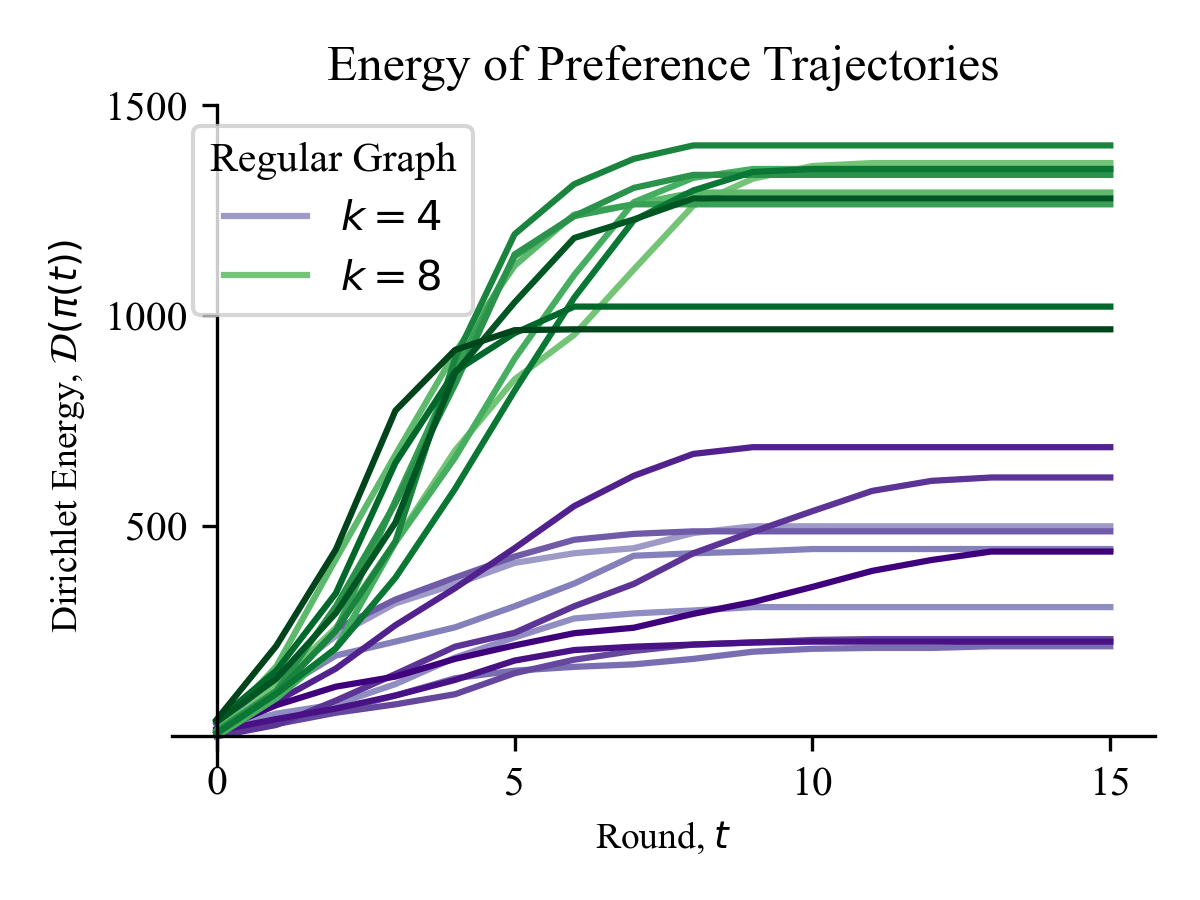
\includegraphics[width=\textwidth]{code/plots/experiment_2_4_plot.png}
    \caption{$k=4,8$; join update rule.}%
    \label{fig:experiment_2_4}
\end{subfigure}
\begin{subfigure}[b]{0.5\textwidth}
    \centering
    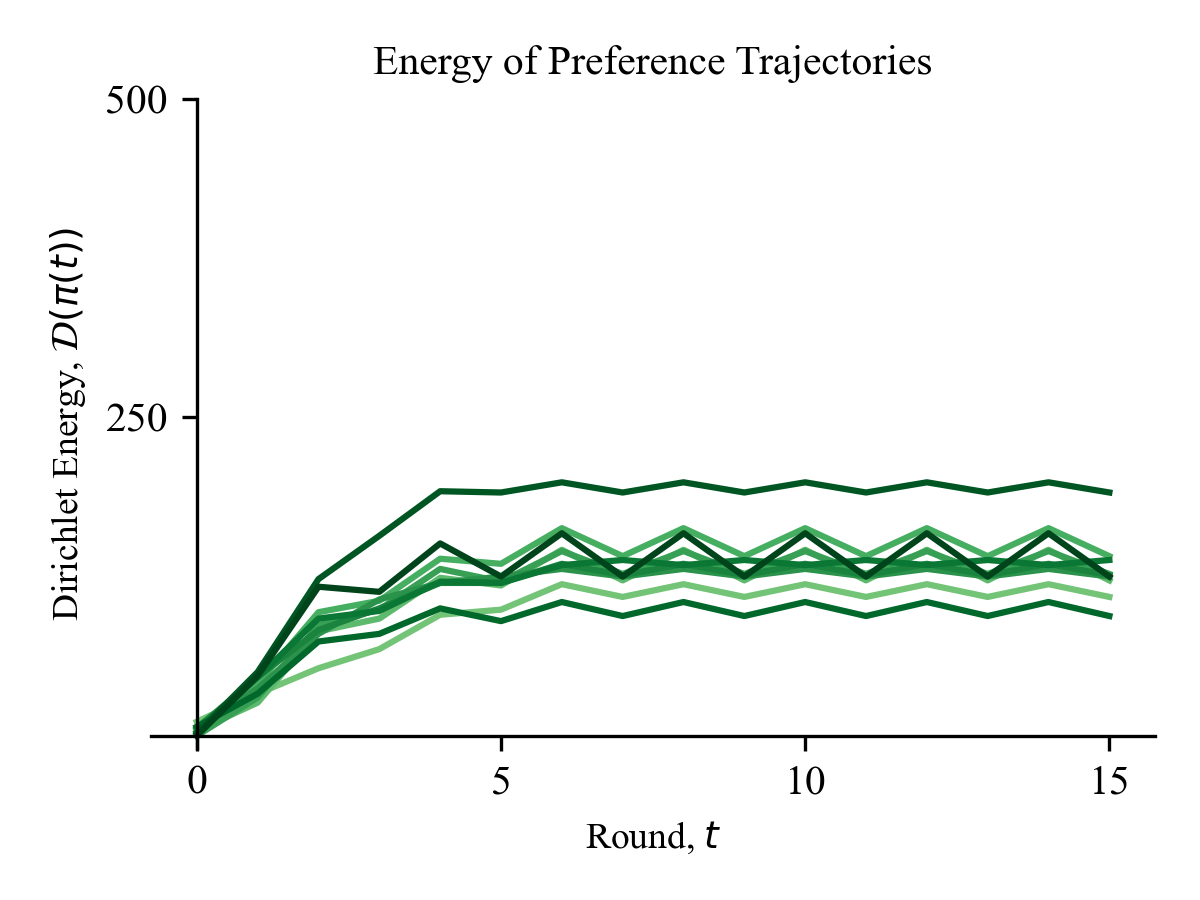
\includegraphics[width=\textwidth]{code/plots/experiment_6_plot.png}
    \caption{$k=2$; posterior update rule.}%
    \label{fig:experiment_5}
\end{subfigure}
\caption{Dirichlet energy $\D(\cdot)$ of trajectories with join update rule (a) or posterior update rule (b) and $r$-median aggregation rules (for random $r$). Trajectories of preference dynamics supported on $k$-regular graphs (for various $k$) with various initial profiles. }
\end{figure}


\paragraph*{Discussion of results}
In the first experiment (Fig.~\ref{fig:experiment_2_4}), every trajectory converged to a stable preference profile, echoing Proposition \ref{prop:inflationary}. For each $k$, the Dirichlet energy was mostly non-increasing each round. The choice of the join update function reflected a higher level of disagreement between agents. Graphs with higher connectivity (higher $k$) generally converged faster and converged to preference profiles with higher Dirichlet energy. We were surprised that trajectories tended to cluster into stable preference profiles with a similar level of total disagreement, i.e. Dirichlet energy. Perhaps several profiles in the lattice of stable profiles (Theorem \ref{thm:complete-lattice}) have similar levels of Dirichlet energy. In the second experiment (Fig~\ref{fig:experiment_5}), period-$2$ cycles occur for every initial profile. To our surprise, while we expected cycles with different energies, the energy level between the alternating profiles of a particular cycles is relatively small.


\section{Discussion}
\label{sec:discussion}
%%%%%%%%%%%%%%%%%%%%%%%%%%%%%%%%%%%%%%%%%%%%%%%%%%%%%%%%%%%%%%%%%%%%%%%%%%%%%%%%%%%%%%%%%%

\paragraph*{Fixed point algorithms}x
Proposition \ref{prop:initial-conditions} implies that you can compute fixed points by, first, querying initial conditions until $\boldsymbol{\pi(0)} \in \Pre(F) \cup \Post(F)$, then, computing trajectories until they converge. It is not clear if you would achieve better complexity than exhaustive search of $\Pref(\A)^N$ by this method. Is it possible to find an aribitrary fixed point in some other way? Suppose $\P = \{1,2,\dots,n\}$ with the standard order. For the product lattice $\P^d$, there is an inductive algorithm on $d$ for computing fixed points of a monotone function $f: \P^d \to \P^d$ running in $O(\log^d n)$ time \cite{?}. The base-case, finding a fixed point of $f: \P \to \P$, is equivalent to binary search: Initialize $m = \lceil n/2 \rceil$. If $f(m) < m$, restrict $f$ to $\{1,2,\dots,m-1\}$. If $f(m) > m$, restrict $f$ to $\{m+1,m+2,\dots,n\}$. Otherwise, $f(m) = m$ and you are done. In our case, a similar inductive algorithm is not possible, because, in the base case $f: \Pref(\A) \to \Pref(\A)$, the binary search method would require the information order on $\Pref(\A)$ to be a chain, i.e.~totally ordered. To the best of our knowledge, there are no algorithms for computing fixed points of finite lattices, in general, besides exhaustive search.

\paragraph*{Metapreferences}
Suppose we are able to call to an oracle that produces an arbitrary fixed point, i.e.~a stable preference profile. Is this preference profile desirable? In future work, we want to prune the set of preferences in such a away that stable preferences are acceptable to human supervisors. Critical in this line of reasoning is the notion of a \emph{metapreference},  or higher-order preference, a notion of a preference over preferences. Formally, an arbitrary ordering on a set of preferences \cite{lutskanov2015}, a narrower class of metapreferences can be represented by utility functions on a set of preference relations, which can be interpreted as measuring the cost or benefit of a preference to the agent as well as the supervisor \cite{munger2019}. Utility functions representing a given metapreferene relation are not unique, i.e.~utility functions capture more than the relative order of preferences. The values of metapreference utilities reflect the degree to which adding additional relations $a \prefers b$ will increase or decrease utility. If every agent has a utility function specifying the cost or benefit of holding every possible preference, maximizing
\begin{align}
    \max_{\profile = (\pi_1,\pi_2,\dots,\pi_N)} \sum_{i=1}^N v_i(\pi_i), \label{eq:dist-opt}
\end{align}
is equivalent to finding the preference profile that is the most acceptable to the supervisor.



\paragraph*{Switching topology}
We assumed that the topology is fixed so that agents interact with the same set of neighbors in each round. We want to relax this assumption so that we can model preference dynamics in systems with more complex patterns of interaction. Suppose the topology of the network is not fixed, and switches according to $\G(t) = \left(\N, \E(t)\right)$. If agents update preferences according to a heterogeneous but fixed-in-time message-passing schema \eqref{eq:message-passing}, then the global dynamics $\profile(t+1) = F_t\left( \profile(t)\right)$ is now a time-variant system. While it is clear that the time-invariant solutions can be identified as intersections and unions of $\{\Fix(F_t)\}_{t = 0}^{\infty}$, these solutions no longer have the structure of a lattice (Theorem \ref{thm:dynamics}), in general. Furthermore, it is not clear what constraints on the connectedness of $\G(t)$ need to be imposed in order to guarantee  non-emptiness of $\SS$ or other desirable properties.

\bibliographystyle{ieeetr}
\bibliography{IEEEabrv,biblio}

\appendix

\subsection*{Proof of Theorem \ref{thm:complete-lattice}}

% \subsection*{Proof of Proposition \ref{prop:join}}




\end{document}
